\documentclass[11pt]{article}

\usepackage[margin=1in]{geometry}
\usepackage{graphicx}
\usepackage{caption}
\usepackage{float}
\usepackage{booktabs}
\usepackage{amsmath}

\captionsetup{font=small, labelfont=bf, justification=raggedright,
              singlelinecheck=false}

% Overleaf: upload both figure PDFs anywhere in the project.
\graphicspath{{julia_descriptive/plots/}{plots/}{./}}

\title{Essay 2 progress report:\\
US institutional ownership, Chinese supply-chain exposure,\\
and US--China tension}
\author{Prepared for Stefano Cassella and Emanuele Rizzo}
\date{4 August 2026}

\begin{document}

\maketitle

\section{The question, and the answer}

The essay asks one thing. When US--China tension rises unexpectedly, do
US institutional investors reduce their portfolio weight in European-listed
firms with Chinese supply-chain links, relative to non-US investors holding
the same firm in the same quarter?

The comparison lives inside a firm-quarter. Two
holder groups, US and non-US, hold the same stock at the same date. Anything
that happens to the firm happens to both. The firm's China exposure, the
tension shock itself, and the interaction of the two are all common to the
cell and drop out. What remains is the differential response of one investor
group. Political pressure and reputational exposure to a China story fall on a
US asset manager, not on a Dutch pension fund holding the same share. If geopolitics moves portfolio equity through the
investor side rather than through prices, this design should see it.

It does not. On the current panel the triple-interaction coefficient is
$\beta_3 = -0.53 \times 10^{-6}$ with a two-way clustered standard error of
$1.74 \times 10^{-6}$, over 347,690 firm-group-quarter observations. The
clustered $p$-value is 0.763 and the randomization-inference $p$-value is
0.815 under free permutation and 0.829 under circular shift. The point estimate
is smaller than its own standard error, a $t$ of $-0.3$. It sits in the
hypothesized direction and is far too small to matter.

Two things have changed since the descriptive note I sent you. I rebuilt the
supply-chain exposure measure in July (Section~4a). Then, this week, I found a
data error in the holdings ETL that had been running since the start of the
project (Section~4b). The second one matters more than any robustness check in
this report, and it also means the claim I made in that note, that 2022 was the
deepest drawdown in the sample, was wrong. Section~5 retracts it.

\section{Data and measurement}

\paragraph{Ownership.} FactSet Ownership v5. A raw row is one fund's position
in one security at one report date, valued in US dollars. I aggregate to firm
$\times$ holder group $\times$ quarter, where the holder group is US or
non-US by the fund's FactSet registration domicile. For firm $i$, group $g$,
quarter $t$: $H_{i,g,t}$ is the group's total dollar position in the firm,
$T_{g,t}$ is the group's total European book, $w_{i,g,t} = H_{i,g,t}/T_{g,t}$,
and the outcome is the backward difference
$\Delta w_{i,g,t} = w_{i,g,t} - w_{i,g,t-1}$. The holdings panel behind this
now carries 208,418,523 fund-security-quarter rows.

Registration domicile is not decision nationality. A US manager's Luxembourg
UCITS vehicle sits in the non-US group even though the allocation decision and
any political-pressure channel are American. That is treatment-group
misclassification and it compresses $\beta_3$ toward zero. Regrouping by
management-company ultimate parent is on the list and not done.

Raw FactSet records only held positions, so a zero holding is a missing row,
not a zero. Since the hypothesis is about moving toward zero, I build the full
Cartesian grid of holdings-observed European issuers $\times$ quarters
$\times$ two groups and zero-fill. An exit then appears as
$\Delta w = -w_{t-1} < 0$ instead of vanishing from the data.

\paragraph{Supply-chain links.} FactSet Revere records directed firm-to-firm
relationships with counterparty country and disclosure-based start and end
dates. Exposure is
\[
\mathrm{CN}_{i,t} \;=\; \frac{L^{\mathrm{CN}}_{i,t}}{L_{i,t}},
\]
where $L_{i,t}$ counts firm $i$'s active customer and supplier edges at the
close of quarter $t$, and $L^{\mathrm{CN}}_{i,t}$ counts those whose
counterparty is Chinese. Edges are counted symmetrically: the firm may sit on
either side, and the Chinese side is the union of firm-as-source and
firm-as-target. The measure enters lagged one quarter. Home-region classification is point-in-time, so
there is no look-ahead in the exposure.

Competitor links and the partnership family (joint venture, licensing,
manufacturing, marketing) are excluded from both numerator and denominator.
They were 14.85 and about 21 percent of Chinese edges respectively. A rival in
Shenzhen is not an input dependency, and leaving those edges in inflated the
denominator for firms whose China contact was competitive rather than
transactional. This restriction also aligns the regression measure with the
descriptive figure, which was always built on customer and supplier links.

A firm with no supply-chain edges at all gets a missing value, never a zero.
Those firm-quarters sit in a documented missing bucket rather than in the
low-exposure arm. That rule, plus the customer-supplier restriction and the
one-quarter lag, is why the estimation universe of 6,867 firms is so much
smaller than the 12,791 European securities in the holdings data. I did not
re-derive the intermediate steps of that cascade on the corrected panel this
cycle.

\paragraph{Shock.} The bilateral AI-driven geopolitical risk index of
Iacoviello and Tong (2026), monthly, directional \texttt{USA|China}. I fit an
AR(1) in levels by OLS on the monthly series ($\hat{a} = 0.694$,
$\hat{b} = 0.657$, $n = 796$ months, $R^2 = 0.43$) and take the residual at the
final month of each quarter. $S_t > 0$ is an unexpected escalation. Over the 82
estimation quarters the shock has mean 0.167 and standard deviation 2.578.

\paragraph{The estimation panel.} 348,156 rows, 6,867 firms, 82 quarters
(2003Q3--2023Q4), balanced 50/50 across the two groups. A row is one firm, one
holder group, one quarter.

\section{Design}

The estimating equation is the four-coefficient form used in the cross-border
bank-lending literature, ported from loans to portfolio equity:
\begin{equation*}
\begin{split}
\Delta w_{i,g,t} \;=\;& \beta_0 \, \mathrm{US}_g
\;+\; \beta_1 \, (\mathrm{US}_g \times S_t)
\;+\; \beta_2 \, (\mathrm{US}_g \times \mathrm{CN}_{i,t-1}) \\[2pt]
&\;+\; \beta_3 \, (\mathrm{US}_g \times \mathrm{CN}_{i,t-1} \times S_t)
\;+\; \alpha_{i,t} + \gamma_{g,t} + \mu_{i,g} + \varepsilon_{i,g,t}.
\end{split}
\end{equation*}

Three pairwise fixed effects on $\{$firm, group, quarter$\}$. The firm
$\times$ quarter effect $\alpha_{i,t}$ absorbs the levels of
$\mathrm{CN}_{i,t-1}$, $S_t$ and their interaction, along with everything else
specific to that firm in that quarter, including any price move. The group
$\times$ quarter effect $\gamma_{g,t}$ absorbs $\beta_0 \mathrm{US}_g$ and
$\beta_1 (\mathrm{US}_g \times S_t)$, so any
quarter in which US money as a whole leaves Europe is differenced away. The
firm $\times$ group effect $\mu_{i,g}$ absorbs a permanent US-versus-non-US
tilt toward each firm. Only $\beta_2$ and $\beta_3$ survive. $\beta_3$ is the
third cross-derivative $\partial^3 \Delta w / \partial \mathrm{US} \,
\partial \mathrm{CN} \, \partial S$, and the hypothesis of Section~1, which I
label H2.1, predicts $\beta_3 < 0$. Saturating this way costs 466
singleton observations, leaving $N = 347{,}690$, 6,634 firm clusters and 82
quarter clusters.

Standard errors are two-way clustered on firm and quarter. Quarter clustering
is the binding dimension: $S_t$ is one common time series, so the effective
number of independent shock draws is 82, not 347,690.

I do not treat the clustered $p$-value as the arbiter. Randomization inference
(RI) is. Three reasons. First, with 82 quarter clusters the design sits close
enough to the small-$G$ region that the cluster-robust variance is fragile. In
practice \texttt{reghdfe}'s Cameron-Gelbach-Miller repair fired in about a
dozen specifications this cycle, and the standard positive-definiteness check
does not flag that. Second, several outcomes are fat-tailed, and one of them
badly so (Section~7a). Third, the local-projection outcomes overlap in time by
construction, so their errors are serially dependent whatever the cluster
structure says.

Randomization inference permutes the 82 quarterly shock values, holds the
panel fixed, and re-estimates. The shock is measurably persistent at quarterly
frequency (first-order autocorrelation $+0.271$, Ljung-Box $p = 0.0125$ at lag
1 and $0.0228$ at lag 4), so free permutation is not exchangeability-safe and
is anti-conservative on cumulative outcomes. The reported arbiter is therefore
the circular shift, which preserves the serial structure across 81 non-trivial
rotations. I run moving-block permutation and a within-family maximum-$|t|$
correction alongside it wherever a horizon family creates multiplicity.

\section{Two corrections along the way}

\subsection*{4a. The exposure denominator}

Until July the China share counted every relationship type in both numerator
and denominator. Restricting to customer and supplier edges moved the
high-exposure cutoff, defined as the median of strictly positive lagged
exposure, from 0.0476 to 0.0625, and cut the estimation universe from 7,928 to
6,854 firms. The firms that left are those whose only Chinese contact was a
competitor or partner tie. The headline moved from $+1.80 \times 10^{-6}$
($p = 0.35$) to $+2.75 \times 10^{-6}$ ($p = 0.110$). The measure is cleaner
and the estimate larger. It is still null. One marginal cell in the firm-level
ladder specifications lost its star.

\subsection*{4b. The holdings snapshot}

This is the important one.

The ETL step that builds the quarterly holdings panel kept rows whose
\texttt{REPORT\_DATE} equalled the calendar quarter-end exactly. FactSet
shifts a fund's report date to the prior business day when the quarter-end
falls on a weekend. Not every fund shifts. So on a Saturday quarter-end the
file kept the funds that stamped the Saturday and silently dropped the funds
that stamped the Friday.

The hole is large and it is concentrated. Fund coverage on weekday quarter-ends
runs 86 to 87 percent over 2016--2023. On 2022-12-31, a Saturday, it was
58.4 percent. On 2023-09-30, also a Saturday, 38.6 percent.

A 40 percent coverage hole would be tolerable if it were symmetric across the
two arms, because group $\times$ quarter fixed effects would absorb it. It was
not symmetric. On 2022-12-31 the funds the old rule dropped were 25 percent
US-domiciled against 21 percent among the funds it kept. A group-composition
shift that varies quarter by quarter moves the within-firm-quarter US minus
non-US difference itself, which is exactly the object $\beta_3$ is built from.

\paragraph{The fix.} For each fund and security, take the latest report on or
before the quarter-end within a window of $W$ calendar days, stamp it to the
quarter-end, and keep the actual report date and the gap as provenance. I set
$W = 10$. The choice sits on a measured coverage plateau rather than on a
result: marginal coverage gained is $+7.18$pp going from $W = 0$ to $W = 3$,
then $+0.29$, $+0.09$ and $+0.11$pp at $W = 7$, $10$ and $14$. A month-wide
window ($W = 31$) buys another 7.95pp but only by importing genuinely stale
positions, 28.4 percent of its rows sitting more than fourteen days from the
quarter-end.

\paragraph{Gate evidence.} The new holdings panel has 208,418,523 rows against
186,800,295 before, and the old panel is exactly the zero-gap subset of the
new one, bit-equal on those rows. The weekday-versus-weekend coverage gap falls
from 22.3 to 4.2 percentage points over the full sample, and from 34.0 to 1.6
in 2016--2023. The US-share selection tilt, which is the bias channel, falls
from $-3.41$pp to $+0.01$pp and is flat in every era. The shock series is
bit-identical before and after on all 265 quarters, and the exposure and shock
columns of the grid are frozen on all 2,548,600 common cells, so exactly one
input moved. The estimation panel goes from 347,952 rows and 6,854 firms to
348,156 and 6,867, and the 204 extra rows are exactly the exposed cells of the
firms that newly enter.

I am disclosing two residual problems rather than fixing them. The coverage gap
does not close to zero: it stops at 4.2pp because the 1999--2005 ramp-up era
sits at 11.3pp, and no choice of $W$ repairs that, since it is a property of
early FactSet coverage. And about 10.4 percent of rows now carry roughly one
day of price drift relative to the quarter-end, 21.6 million of 208.4 million,
because a shifted fund is valued at its own report date. Ninety percent of
those gaps are one or two days. That is a real cost of the as-of rule. It is
small against a 40 percent coverage hole.

\section{What the correction did to the results}

\paragraph{The figure first.} Figure~\ref{fig:us_holdings} is the series I sent
you. Real year-over-year growth in US institutional holdings of European equity
in 2022Q4 was $-42.8$ percent on the old panel and is $-25.9$ percent on the
corrected one. The 2009Q1 trough is unchanged to the last digit at $-39.7$
percent, because
31 March 2009 was a Tuesday. So the ranking reverses. The deepest real
drawdown in the sample is the financial crisis, not 2022. I wrote you the
opposite, and I withdraw it. Nineteen of the 76 plotted aggregate quarters move
by more than two percentage points. The largest are 2014Q2 ($+100.0$ to
$+32.5$) and 2013Q2 ($-21.7$ to $+18.2$). The ones that carry interpretation
are 2023Q3 ($-1.0$ to $+29.1$) and the Covid quarter 2020Q1 ($+0.7$ to
$-15.5$), the latter entirely through its base quarter, since 2019Q1 ended on
a Sunday. Two other statements in that paragraph of the note also fall. The
worst quarter of 2020 is 2020Q1 at $-15.5$ percent, not $-2.1$ percent, so
Covid does register. And end-2023 real holdings stand at 2.3 times the 2007
peak, not 1.8. In levels
the real book still peaks at \$2.21 trillion (2020 dollars) in 2021Q4, but the
end-2023 value rises from \$1.52 to \$1.98 trillion. In nominal terms the
2022Q4 European book goes from \$1.457 to \$1.892 trillion and its
year-over-year change from $-39.2$ to $-21.1$ percent.

Figure~\ref{fig:china_links} is unaffected by construction, since numerator and
denominator come from the same relationship file, and the regenerated figure
confirms it (caption).

\paragraph{Then the regressions.} Table~\ref{tab:prepost} lists every cell that
moved materially. The headline goes from $+2.75 \times 10^{-6}$ ($p = 0.110$,
RI $0.31$) to $-0.53 \times 10^{-6}$ ($p = 0.763$, RI $0.83$).

\begin{table}[H]
\centering
\small
\caption{What the holdings correction did. $p$-values are two-way clustered on
firm and quarter. Coefficients are $\beta_3$ in units of $10^{-6}$ of
portfolio weight, except the country-pair row, which reports $\beta_1$, and
the last row, whose outcome is the shares-outstanding flow and is in its own
units. The local-projection rows use the firm $\times$ quarter and group
$\times$ quarter set. The risk-set sample keeps firm-quarters in which at least
one group holds the firm in that quarter or in the quarter either side,
retaining both group rows; the spell-boundary sample keeps held quarters plus
the single zero quarter immediately before an entry and after an exit, dropping
the never-held interior.}
\label{tab:prepost}
\begin{tabular}{lrrrr}
\toprule
 & \multicolumn{2}{c}{Before} & \multicolumn{2}{c}{After} \\
\cmidrule(lr){2-3}\cmidrule(lr){4-5}
Specification & $\beta_3$ & $p$ & $\beta_3$ & $p$ \\
\midrule
Headline, three pairwise FE      & $+2.746$ & 0.110 & $-0.528$ & 0.763 \\
Firm$\times$qtr $+$ group$\times$qtr only & $+2.081$ & 0.151 & $-1.073$ & 0.557 \\
Local projection, cumulative $h=1$ & $+2.850$ & 0.017 & $-1.248$ & 0.599 \\
Local projection, cumulative $h=2$ & $+5.030$ & 0.003 & $+0.385$ & 0.849 \\
Four-group, US active vs non-US active & $+2.789$ & 0.069 & $-0.706$ & 0.684 \\
Risk-set sample, firm$\times$qtr $+$ group$\times$qtr & $+3.26\phantom{0}$ & 0.151 & $-1.730$ & 0.544 \\
Spell-boundary sample            & $+4.38\phantom{0}$ & 0.441 & $-2.623$ & 0.547 \\
Country-pair $\beta_1$ (US $\times S_{c,t}$) & $+22.2\phantom{0}$ & 0.086 & $-1.361$ & 0.910 \\
Ownership flow, raw (share of shares out.) & $+0.00089$ & 0.0001 & $-0.0361$ & 0.237 \\
\bottomrule
\end{tabular}
\end{table}

Three things follow.

The null survives and deepens: the clustered $p$-value moves from 0.11 to 0.76.

Before the correction almost every specification in the project produced a
small positive $\beta_3$, wrong-signed for the hypothesis but suspiciously
consistent. Those positives are gone. The signs are now mixed and the
magnitudes smaller. The old positive lean was substantially the
weekend-composition artifact. Weekend quarters under-counted US holdings, so
the following quarter's recovery read as US buying, and that fake buying loaded
onto the interaction through the composition tilt. I have not isolated that
channel beyond the measured tilt and the sign flip, so the reading is an
inference from those two facts and not a separate test.

The last surviving rejection dissolves. Before the correction the cumulative
four-quarter local projection rejected at 0.039 under free permutation and was
the only cell in the project to do so. It is now 0.066 free and 0.122 under the
arbiter. That cell had already been killed independently by the serial-robust
inference work that preceded this rebuild, so it is now dead twice over, once
on inference and once on data.

\section{How hard the null has been pushed}

\paragraph{Outcome families.} The intensive margin was never going to be the
whole story, since a group-level weight barely moves when five of ten US funds
liquidate. Table~\ref{tab:families} therefore runs the same specification
across value, stake and count outcomes. The extensive-margin outcomes are the
ones the divestment literature says should signal first. They are null too.

\begin{table}[H]
\centering
\small
\caption{Outcome families, all on the corrected panel and the same
three-pairwise specification. RI is the circular-shift arbiter, except the two
Stake rows, which are free-permutation $p$-values (the flow RI engine has no
circular-shift leg). The
winsorized flow column is the pre-committed main specification for the
stake outcome; the raw column is discussed in Section~7a.}
\label{tab:families}
\begin{tabular}{llrrr}
\toprule
Margin & Outcome & $\beta_3$ & clustered $p$ & RI $p$ \\
\midrule
Value    & $\Delta$ portfolio weight (headline) & $-5.28 \times 10^{-7}$ & 0.763 & 0.829 \\
Stake    & Flow, share of shares out., winsorized & $+7.48 \times 10^{-5}$ & 0.827 & 0.913 \\
Stake    & Flow, raw (outlier-dominated)         & $-3.61 \times 10^{-2}$ & 0.237 & 0.021 \\
Breadth  & $\Delta$ normalized holder breadth    & $+2.20 \times 10^{-5}$ & 0.568 & 0.573 \\
Breadth  & $\Delta$ holder count                 & $-1.45$                & 0.167 & 0.220 \\
Exit     & Position terminated, given both held  & $+1.42 \times 10^{-3}$ & 0.704 & 0.683 \\
Entry    & Position initiated, given neither held & $-6.62 \times 10^{-4}$ & 0.780 & 0.829 \\
\bottomrule
\end{tabular}
\end{table}

\paragraph{Shock construction.} The baseline shock has three known defects: it
is serially correlated at quarterly frequency, it uses only the US-initiated
direction of a bilateral index, and its AR was fit on the full sample including
years after the panel ends. I built ten alternative constructions, crossed with
the direction axis. Before any regression ran I wrote the selection rule into
the builder header: pick the no-look-ahead variant with the whitest quarterly
residual by Ljung-Box at lag 4, report direction as a parallel column set,
never select on outcomes. Then I ran the whole menu.

None of the twelve randomization-inference columns rejects at 5 percent under
either free permutation or circular shift. The smallest arbiter $p$ in the
entire menu is 0.244. Two columns do cross 0.05 on clustered standard errors,
and both dissolve under the arbiter. They correlate 0.892 with each other, so
they are closer to one column than to two. The preferred variant's one-quarter
lead specification also flips sign, which a real lagged disengagement effect
would not do.

Two constructions actually whiten the residual: take a quarterly mean first and
fit an AR(1) to it, or difference the monthly index first and fit AR(4). The
winner is rule-dependent. The quarterly-mean variant wins on Ljung-Box at lag
4; its lag-8 $p$ of 0.085 is worse than the runner-up's 0.132, and an
autocorrelation-first rule would have selected the differenced AR(4) column
instead. The selected series is whiter, not white. Summing a monthly AR(1)
residual over the quarter is the worst column in the menu. It also carries the
third-lowest clustered $p$-value, which shows what serial correlation does to
clustered inference.

\begin{table}[H]
\centering
\small
\caption{Shock-construction menu, selected columns. $\beta_3$ per one standard
deviation of the respective shock, in units of $10^{-6}$, so the baseline row
is the headline coefficient of Table~\ref{tab:prepost} rescaled to unit shock
variance. The preferred variant was chosen by a rule fixed in writing before
estimation. That winner is rule-dependent, and its residual is whiter but not
white; see the text.}
\label{tab:shockmenu}
\begin{tabular}{llrrr}
\toprule
Variant & Direction & $\beta_3$ & clustered $p$ & RI $p$ (arbiter) \\
\midrule
Baseline, monthly AR(1) level, quarter-end month & USA$|$China & $-1.36$ & 0.763 & 0.829 \\
No-look-ahead refit of the baseline              & USA$|$China & $-1.23$ & 0.784 & 0.866 \\
AR(4) on the differenced monthly index           & USA$|$China & $-2.92$ & 0.443 & 0.573 \\
Within-quarter sum of the AR(4) residual         & USA$|$China & $-6.25$ & 0.026 & 0.280 \\
Quarterly aggregation first, then AR(1) (preferred) & USA$|$China & $-7.56$ & 0.031 & 0.244 \\
Bidirectional sum                                & both        & $+0.45$ & 0.913 & 0.915 \\
Reverse direction only                           & China$|$USA & $+3.98$ & 0.151 & 0.451 \\
\bottomrule
\end{tabular}
\end{table}

\paragraph{Composition alternatives, tested and rejected.} Three stories could
generate an aggregate null out of a real effect. Sell-side and buy-side China
exposure could offset. Split additively, the sell arm is
$-1.96 \times 10^{-6}$ (RI 0.474), the buy arm $+1.01 \times 10^{-6}$
(RI 0.670), and pooling is not rejected, $F(2,81) = 0.77$, $p = 0.465$. Passive
money could dilute active divestment: the pure US-active versus non-US-active
contrast is $-7.06 \times 10^{-7}$ ($p = 0.684$, RI 0.780), essentially the
pooled headline, and the post-2018 window with predetermined fund labels is
$+5.05 \times 10^{-7}$ (RI 0.798). Cutting the 82 quarters into terciles to
look for concentration in large shocks gives $+2.77 \times 10^{-6}$ in the top
tercile (RI 0.848) and $+2.07 \times 10^{-6}$ on the top-minus-bottom contrast
(RI 0.874). With 27 or 28 quarters per bin, the few-cluster problem of the
two-sigma shock dummy I used in the earlier cycle is gone. The permutation
$p$-values in this paragraph are free permutation; the direction, four-group
and tercile engines carry no circular-shift leg.

\paragraph{What bounds the power.} The Russia positive control is the honest
constraint. Running the identical pipeline with Russian supply-chain exposure
and a \texttt{USA|Russia} shock, the coefficient is $-3.87 \times 10^{-6}$ on
the headline specification with a clustered $p$ of 0.018. The sign is right and
the clustered test rejects. Under the arbiter it does not: RI $p = 0.220$. All
eight local-projection horizons after the invasion are negative, and none has a
permutation $p$ below 0.270. So a large, well-dated divestment episode produces
the right sign and still fails design-based inference here. I cannot read the
China null as no effect. The design might also miss a real effect of moderate
size.

The formal version of that statement is the minimum detectable effect. With
$\mathrm{SE}(\beta_3) = 1.743 \times 10^{-6}$, $\sigma_S = 2.578$, and a
representative firm at $\mathrm{CN} \in [0.05, 0.15]$, the 80-percent-power MDE
for a one-standard-deviation shock is $0.63$ to $1.89 \times 10^{-6}$ in
weight-change units. On the stake outcome, using the winsorized standard error
of $3.40 \times 10^{-4}$, it is 1.2 to 3.7 basis points of shares outstanding,
about 2.5 at $\mathrm{CN} = 0.10$. A reallocation larger than that would have
been detected with 80 percent probability. Ruling it out formally is the
equivalence test of Section~8, which has not been run. Two caveats travel with
these figures. The MDE is built from the clustered standard error while
randomization inference is the declared arbiter, and the quarter-end sampling
of the shock is classical measurement error, so the true MDE is somewhat larger
than what is quoted here.

\section{What is still open}

\paragraph{7a. Raw-flow outliers.} The as-of rule recovered positions that the
old panel had dropped, and in a handful of firm-quarters those positions meet a
stale, tiny lagged share count. The result is impossible flow ratios: the
maximum is 1,725 times shares outstanding against a 99th percentile of 0.139,
and kurtosis is about 199,000 where it used to be about 5,000. The raw flow
cells all reject at roughly 0.02 under randomization inference, each at nearly
the same $p$, which is the signature of the same few quarters driving every
one. One decomposition cell implies a quarterly flow of $-107$
percent of shares outstanding per unit of exposure times shock, which is not a
quantity that exists.

Winsorized flow at the 1st and 99th percentiles is the pre-committed main
specification for this outcome, fixed after an earlier episode in which fat
tails drove a result, and not chosen this week. It is unaffected and null
($+7.48 \times 10^{-5}$, RI 0.913), as are all three winsorized decomposition
cells (flow\_r 0.913, flow\_common 0.640, flow\_diff 0.833), together with
their clustered companions. So the substantive
conclusion does not turn on this. Two things do. The co-movement fact I used
when discussing the flow decomposition, that US and non-US flows into the same
firm correlate about $+0.20$, does not survive the rebuild: it is $+0.03$ on
the winsorized high-exposure cut and $+0.01$ on the stable-denominator cut.
I have to rewrite that sentence. And I cannot report the raw column as
informative until a predetermined rule removes the monster cells. The plan is
to extend the existing bad-firm-quarter screen to cover stale denominators,
keyed on the lagged share count rather than on the outcome, so it is not a trim
chosen after seeing which cells are inconvenient.

\paragraph{7b. The four-quarter horizon.} The cumulative four-quarter horizon is
the one place where two valid inference routes disagree. Randomization
inference says null: 0.066 free, 0.122 circular shift, about 0.107 under
moving-block permutation, and 0.056 to 0.062 after the within-family
maximum-$|t|$ correction. A score-based wild cluster bootstrap on quarter
clusters says 0.004. The bootstrap needs quarters to be independent draws. The
shock is measurably serially correlated, so the one assumption the bootstrap
rests on is the one the data deny. Randomization inference stays the arbiter by
the hierarchy I fixed before this cycle, so I report the horizon as not
surviving. I keep the bootstrap number here with its assumption attached rather
than dropping it. The coefficient there is $+6.60 \times 10^{-6}$, positive,
so even taken at face value it points against the hypothesis.

\paragraph{7c. The early-sample coverage gap.} The as-of rule cannot close the
1999--2005 hole, which stays at 11.3 percentage points because early FactSet
coverage is genuinely thin rather than mis-stamped. The estimation sample
starts in 2003Q3, so part of that era is inside the panel.

\paragraph{7d. Sample start.} The natural response to 7c is to re-run the
headline from 2006. That is a decision I would like your view on. It costs ten
of the 82 quarters, and the quarter count is the binding power constraint here.
What it buys is a cleaner coverage regime over a period with almost no
China-tension variation. My prior is that it belongs in
the robustness table and not in the main specification, but I have not run it.

\paragraph{Two smaller watch items.} The within-quarter aggregated shock gives
the lowest non-Russia $p$-value anywhere outside the shock menu of
Table~\ref{tab:shockmenu}: $-1.66 \times 10^{-6}$ at $p = 0.094$. That cell has
no permutation arbiter of its own. Its two-way analogue inflates from 0.097 to
0.235 under free permutation, so I assume this one behaves the same way, and I
am recording that as an assumption rather than a measurement. And the
exit outcome under the two-way fixed-effect companion is negative and
significant at 0.044, meaning US investors exit \emph{less}, while its
three-pairwise primary has the opposite sign and $p = 0.704$.

\section{Where this goes}

As it stands the contribution is measurement and inference discipline more than
a new economic fact. I built a firm $\times$ holder-group $\times$ quarter
panel that sees entry and exit, not only continuing positions, and matched it
to a directed supply-chain network with point-in-time country labels. I then
judge every result against the 82 shock draws that actually identify it. The
report also documents two errors. One of them had been biasing a coefficient
silently for months and would have been invisible in any specification table.
I would rather present that honestly than dress a null in robustness language.

To make the null a claim rather than an absence, the next step is equivalence
testing. Two one-sided tests against a pre-specified economic bound $\delta$
would convert ``we cannot reject zero'' into ``we can reject anything larger
than $\delta$''. The statistical machinery is trivial; choosing $\delta$ is not, and
it is a judgment about what size of reallocation would matter economically. I
would like to fix that number with you rather than pick it myself.

The economics may still be in prices. The companion hypothesis, H2.2, asks
whether high-China-exposure
European firms earn lower abnormal returns around tension episodes regardless
of whether identifiable US selling occurs. That test does not run at quarterly
frequency against 82 draws. It runs at daily or monthly frequency around dated
events: the 2018 tariff rounds, the 2019 Huawei entity-list designation, the
2022 export controls. The power position is much better. It needs
European return data that I have not yet assembled. If the ownership channel is
genuinely flat and the price channel is not, the pair of results is a more
interesting paper than either alone: the firms are repriced and the investor
base does not move.

\begin{figure}[p]
  \centering
  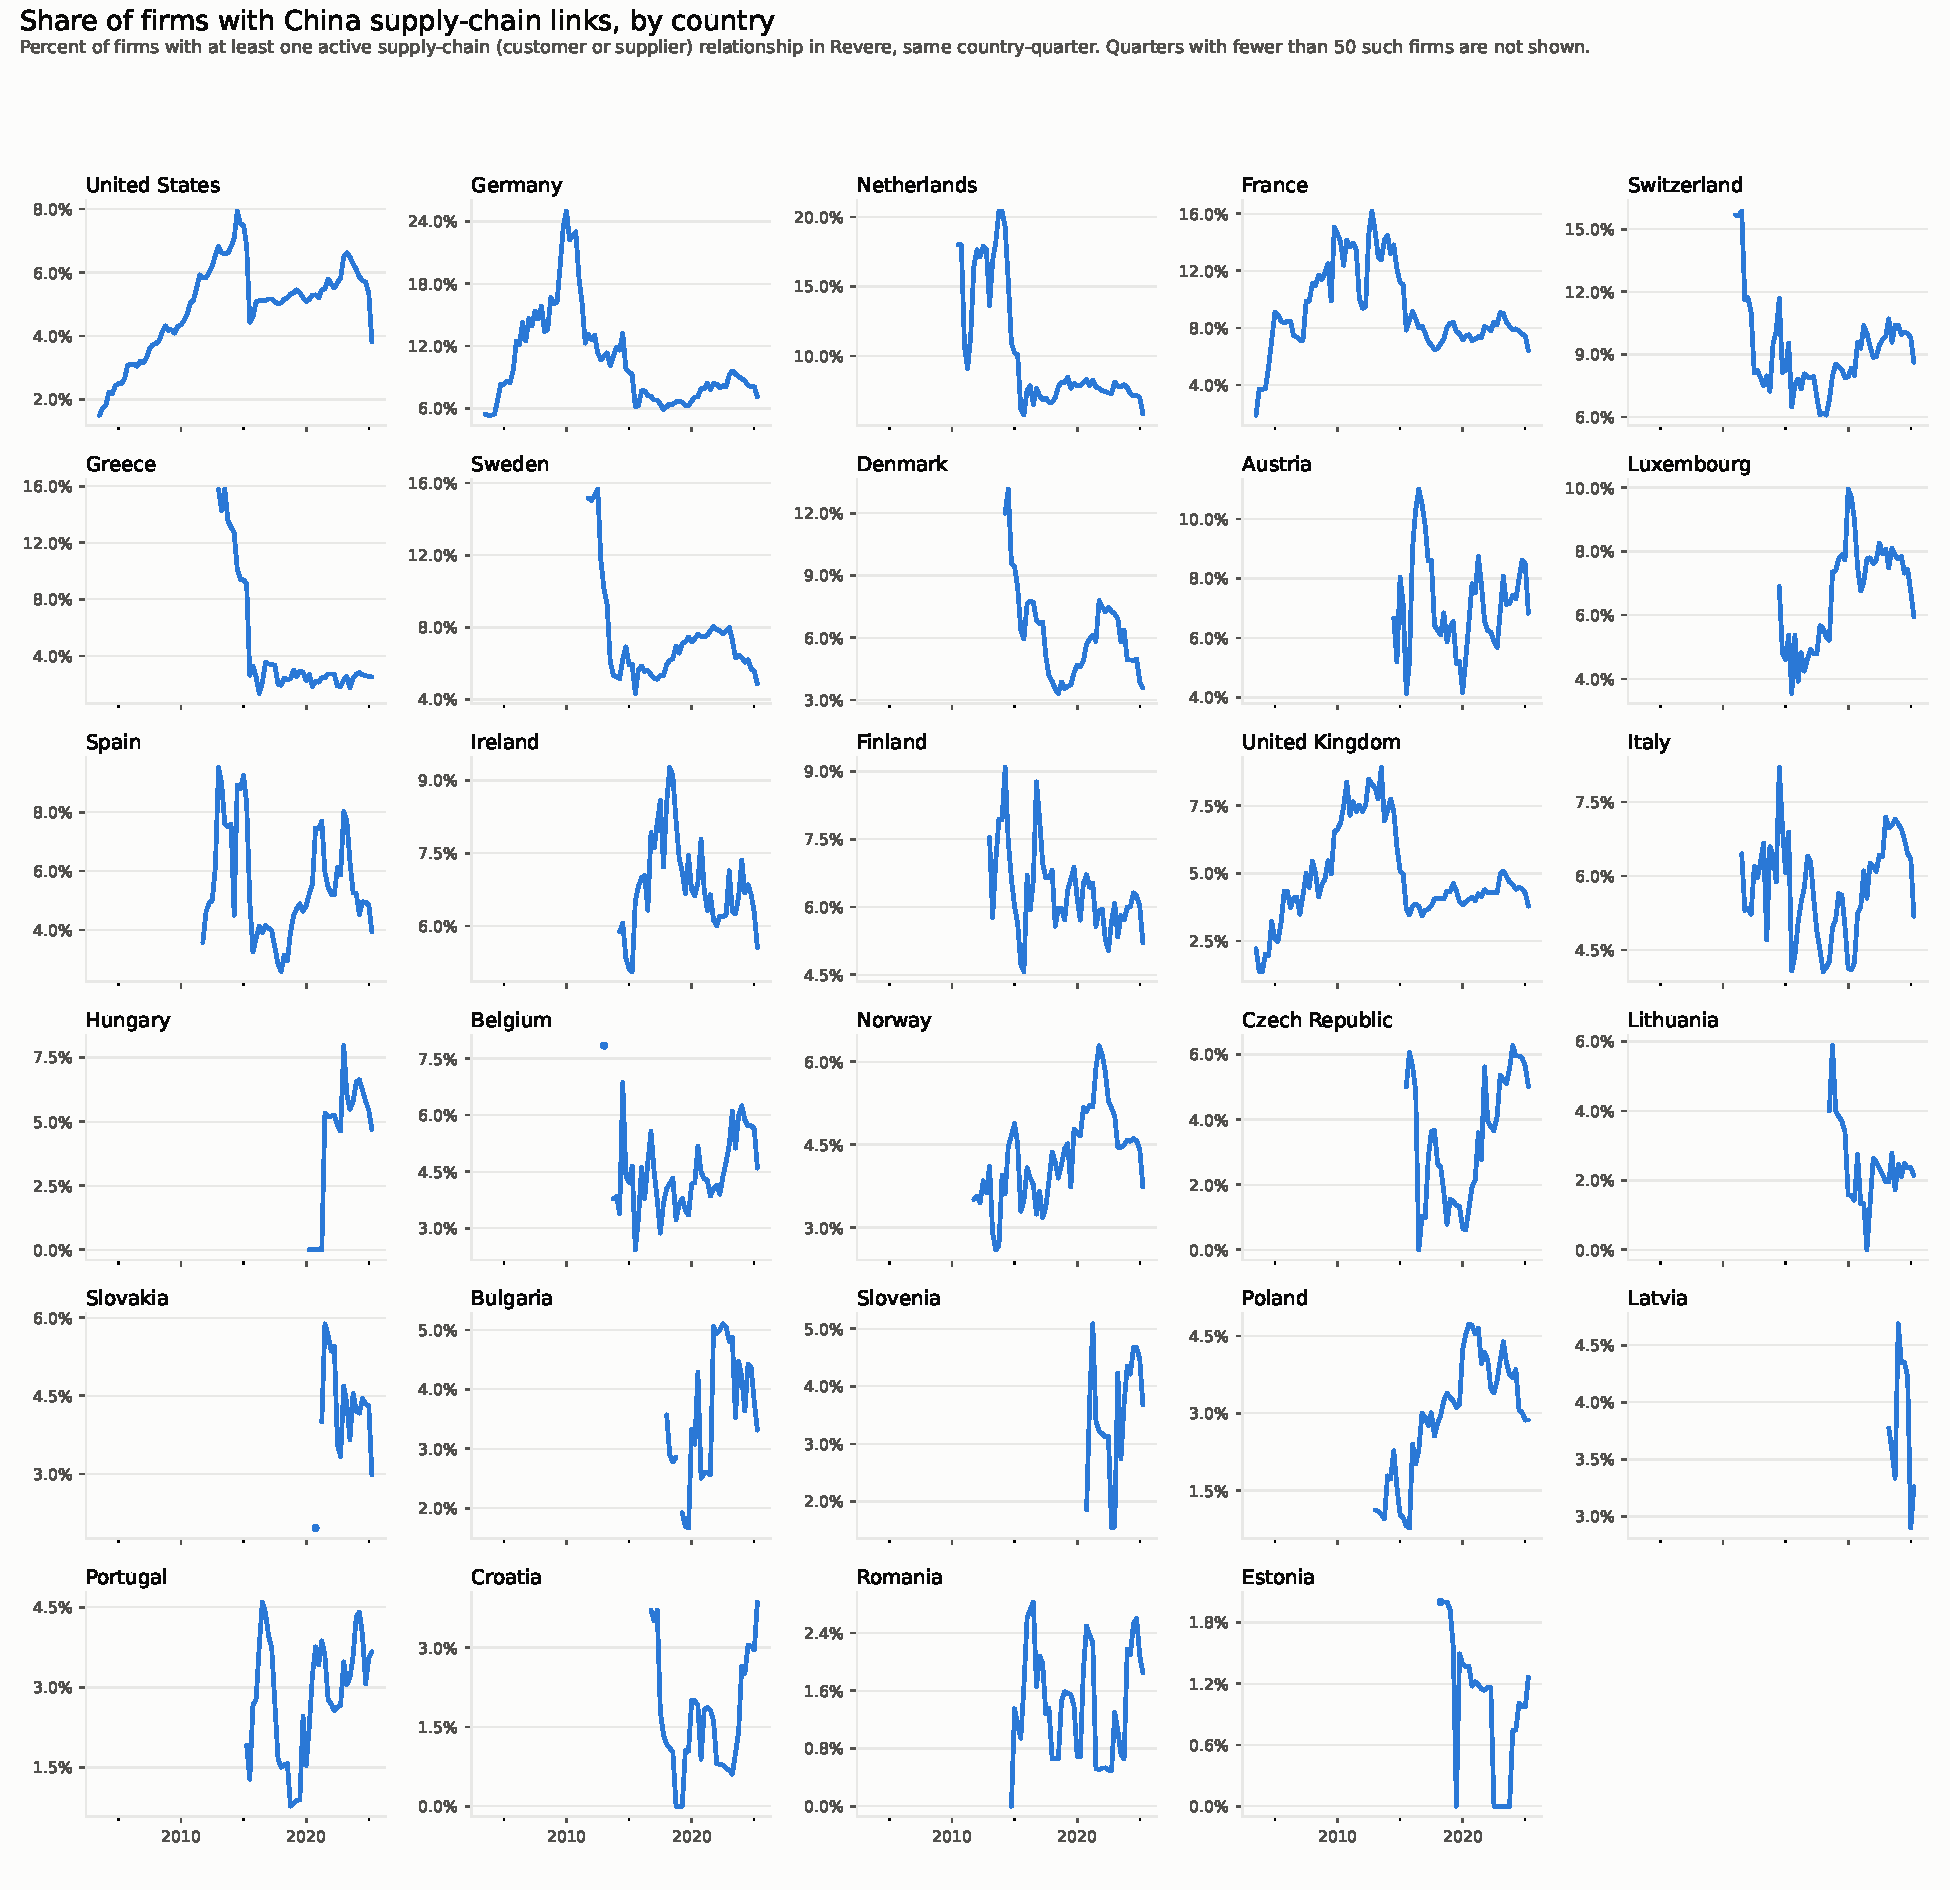
\includegraphics[width=\textwidth]{fig_china_link_fraction.pdf}
  \caption{Share of firms with an active Chinese supply-chain link, by country,
    2003--2025. Each panel is one country; the vertical axis is the number of
    firms with at least one active customer or supplier relationship with a
    Chinese company, as a percent of firms with at least one active customer or
    supplier relationship with any counterparty in the same country-quarter.
    Quarters with fewer than fifty such firms are not shown. This figure is
    unaffected by the holdings correction of Section~4b, because numerator and
    denominator are drawn from the same relationship file; regenerated on the
    corrected pipeline, the largest change anywhere in the figure is 0.22
    percentage points across 7,568 country-quarter cells.}
  \label{fig:china_links}
\end{figure}

\begin{figure}[p]
  \centering
  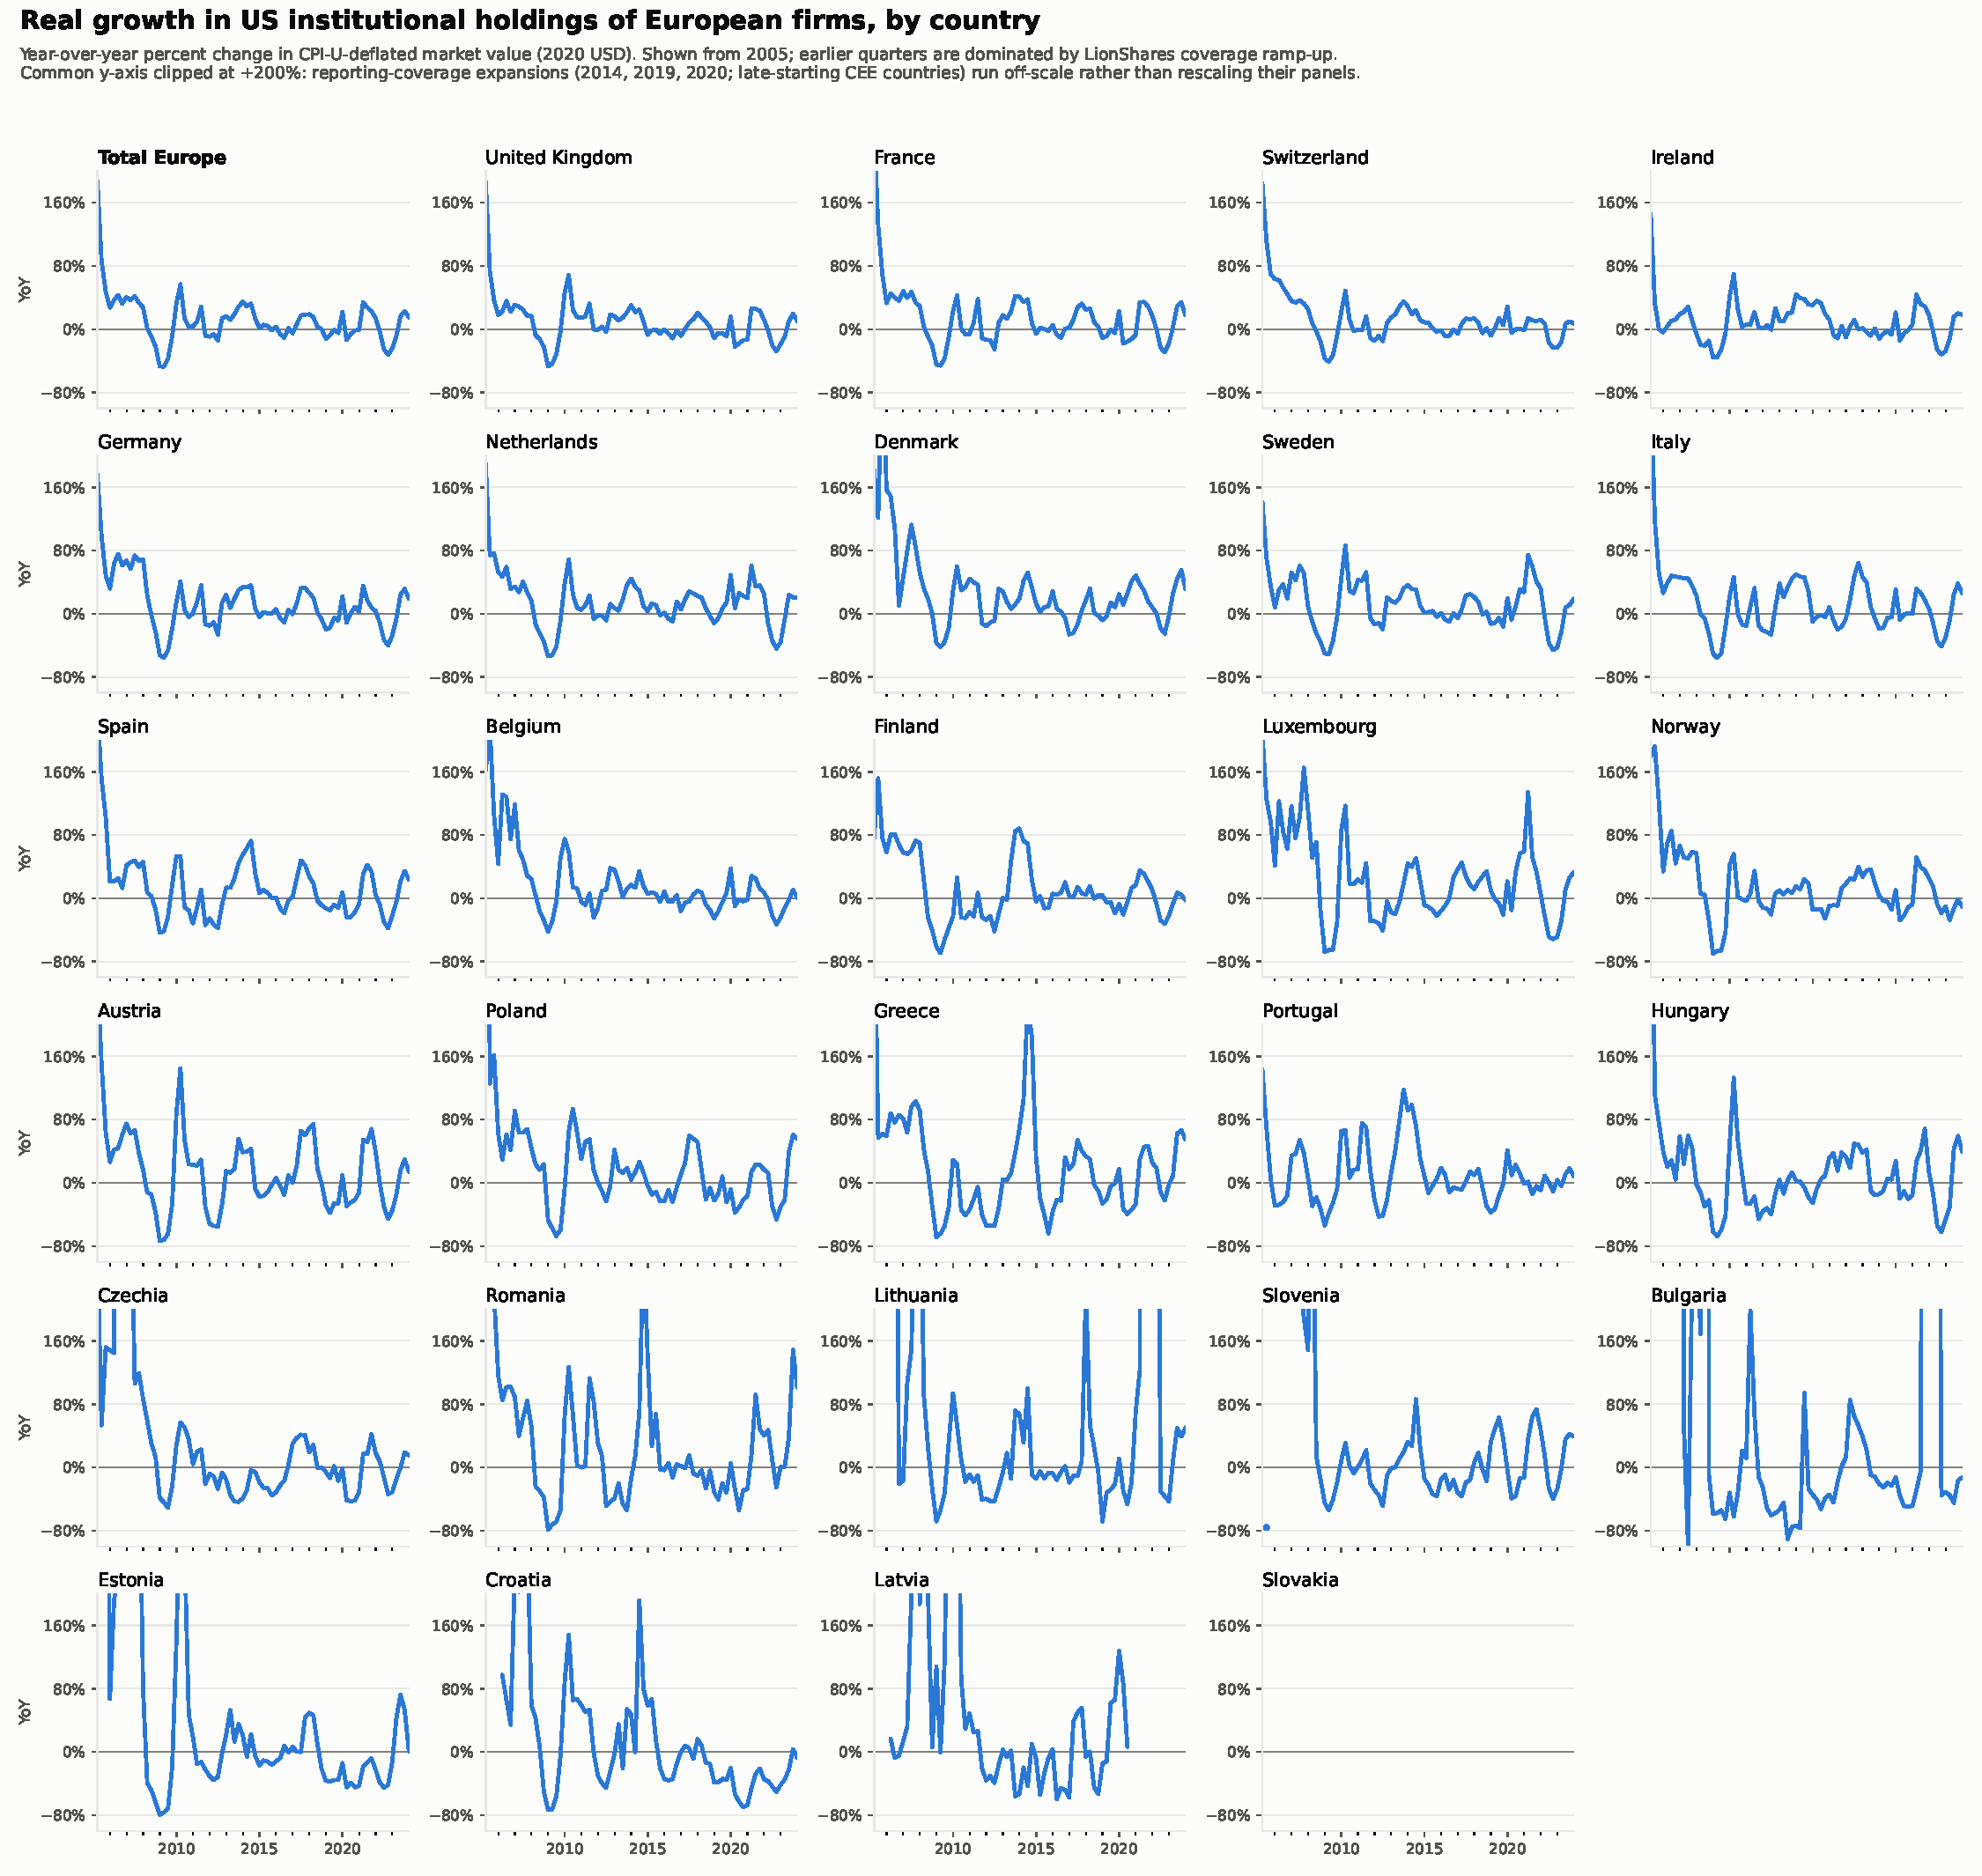
\includegraphics[width=\textwidth]{fig_us_holdings_real_yoy_growth.pdf}
  \caption{Real growth in US institutional holdings of European firms, by
    country, 2005--2023, regenerated after the holdings-snapshot correction of
    Section~4b. Each panel is one country, and the first panel aggregates the
    28-country European sample; the vertical axis is the year-over-year percent
    change in CPI-deflated market value (2020 dollars) of equity held by
    US-domiciled institutional funds, on a common scale capped at $+200$
    percent. \textbf{Correction:} on the earlier panel the 2022Q4 aggregate read
    $-42.8$ percent and appeared to be the deepest real drawdown in the sample.
    That figure was produced by a quarter-end stamping error which dropped a
    large share of reporting funds whenever a quarter ended on a weekend, 41.6
    percent of them in 2022Q4 itself. The
    corrected value is $-25.9$ percent, against $-39.7$ percent in 2009Q1, which
    is unchanged because that quarter ended on a Tuesday. The deepest real
    drawdown in the sample is the financial crisis, not 2022. Nineteen of the
    76 plotted aggregate quarters move by more than two percentage points. The
    largest are 2014Q2 ($+100.0$ to $+32.5$) and 2013Q2 ($-21.7$ to $+18.2$);
    2023Q3 moves from $-1.0$ to $+29.1$ percent and 2020Q1 from $+0.7$ to
    $-15.5$ percent.}
  \label{fig:us_holdings}
\end{figure}

\end{document}
